% ============================================================================
% MScFE 690 | Solution Design Document (one page) | Student Group 17838
% Audience: a manager with no programming background who must sign off.
% Compile: latexmk -xelatex solution_design.tex   (must stay on ONE page)
% The table rows are specification; reword the two short paragraphs and any
% row you want in your own words before submitting.
% ============================================================================
\documentclass[10pt,a4paper]{article}
\usepackage{fontspec}
\IfFontExistsTF{Arial}{\setmainfont{Arial}}{\setmainfont{TeX Gyre Heros}}
\usepackage[margin=1.4cm]{geometry}
\usepackage{booktabs,array,ragged2e,xcolor}
\usepackage{tikz}
\usetikzlibrary{positioning,arrows.meta}
\usepackage{xurl}
\usepackage[hidelinks]{hyperref}
\pagestyle{empty}
\setlength{\parindent}{0pt}
\setlength{\parskip}{3pt}
\definecolor{Ink}{HTML}{283E67}
\newcommand{\head}[1]{\par\vspace{3pt}{\color{Ink}\bfseries #1}\par\vspace{1pt}}

\begin{document}
{\Large\bfseries\color{Ink} Solution Design Document}\hfill{\small Group 17838 | MScFE 690 Capstone}\par
{\small Stop-Loss and Profit-Target Exits for a Cost-Losing Intraday Reversal Rule \quad|\quad Ejike, Odeajo, Kalu}\par
\vspace{2pt}\hrule\vspace{2pt}

\head{1. Business problem}
Traders often add a stop-loss or a profit target to short-term trades, assuming it protects them. Backtests built on one-minute price bars cannot see which price came first inside a minute, and many ignore trading costs. A desk can therefore adopt exit rules that look safe on paper but lose money in practice.

\head{2. What the solution does}
It replays three years of trading days (2021 to 2023) for five large Indian stocks and applies one fixed buying rule. Every trade is then closed three ways, after 15 minutes, at a stop-loss, or at a stop-loss or profit target, with identical entries and sizes. The only difference between the three results is the exit rule. Costs, delays and both possible price orders inside a minute are tested explicitly.

\head{3. Specification}
\small
\begin{tabular}{@{}>{\RaggedRight}p{3.4cm}>{\RaggedRight}p{14.1cm}@{}}
\toprule
Inputs & Instructor minute price files (stocks and NIFTY 50 index), read from Google Drive or a local folder without modification; one declared supplement restores a broken day. \\
Outputs & Tables and charts of average daily profit, worst-day losses (expected shortfall), account drawdown, cost breakdown and sensitivity; a run record with fingerprints of code and data. \\
Fixed settings & Five stocks, one buying rule, 15-minute holding limit, 15 bp trading cost, INR 100,000 reference capital, 60/20/20 split by date. \\
Success criteria & Same inputs give the same outputs; every account balances to within INR 0.0000001; the final test period can be opened only once, after the design is frozen. \\
Platform & Python on Google Colab (no installation needed) or locally in VS Code or Jupyter; one notebook runs the whole study. \\
\bottomrule
\end{tabular}

\head{4. How it works}
\begin{center}
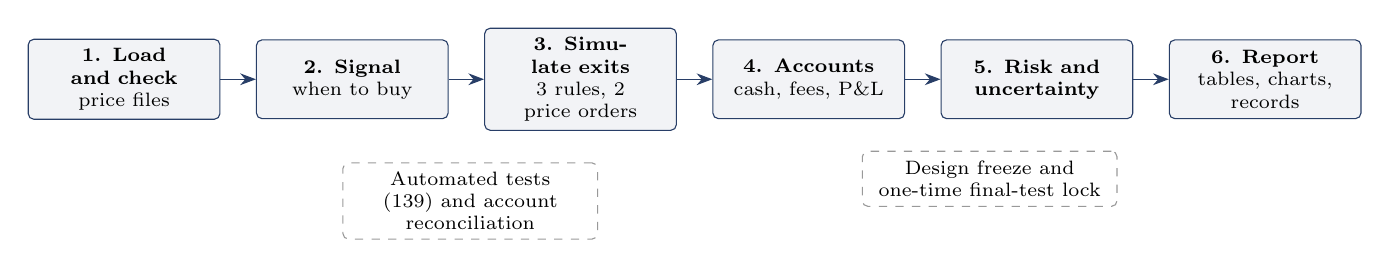
\begin{tikzpicture}[node distance=3mm and 4.5mm, every node/.style={font=\scriptsize,align=center},
  box/.style={draw=Ink,rounded corners=2pt,fill=Ink!6,minimum height=10mm,text width=22mm},
  ctl/.style={draw=black!40,dashed,rounded corners=2pt,minimum height=7mm,text width=30mm},
  arr/.style={-{Stealth[length=2mm]},draw=Ink}]
\node[box] (a) {\textbf{1. Load and check}\\price files};
\node[box,right=of a] (b) {\textbf{2. Signal}\\when to buy};
\node[box,right=of b] (c) {\textbf{3. Simulate exits}\\3 rules, 2 price orders};
\node[box,right=of c] (d) {\textbf{4. Accounts}\\cash, fees, P\&L};
\node[box,right=of d] (e) {\textbf{5. Risk and uncertainty}};
\node[box,right=of e] (f) {\textbf{6. Report}\\tables, charts, records};
\foreach \x/\y in {a/b,b/c,c/d,d/e,e/f} \draw[arr] (\x) -- (\y);
\node[ctl,below=4mm of c,xshift=-14mm] (g) {Automated tests (139) and account reconciliation};
\node[ctl,below=4mm of e,xshift=-6mm] (h) {Design freeze and one-time final-test lock};
\end{tikzpicture}
\end{center}

\head{5. Where each part lives and what it achieves}
\small
\begin{tabular}{@{}>{\RaggedRight}p{3.0cm}>{\RaggedRight}p{5.2cm}>{\RaggedRight}p{8.9cm}@{}}
\toprule
Component & Location in code & What it achieves \\ \midrule
1. Load and check & Notebook: \textit{Load instructor data}; \nolinkurl{src/path_robust/vendor.py} & Reads only the needed files, rejects malformed rows, never fills gaps, applies one declared and checked supplement, records what was used. \\
2. Signal & Notebook: \textit{Signal and sizing} & Flags a stock that fell unusually far behind the index, using past data only. \\
3. Simulate exits & Notebook: \textit{Execution and account balances}; \nolinkurl{src/path_robust/engine.py} & Closes each trade under all three rules and both possible price orders, with costs and slippage. \\
4. Accounts & Notebook: \textit{Session replay and funded segments} & Tracks cash daily and as one continuous account; stops if money would run out. \\
5. Risk and uncertainty & Notebook: \textit{Paired uncertainty and tail risk} & Measures worst-day losses, drawdown and how sure we can be about each difference. \\
6. Report & Notebook: \textit{Save the run and review the freeze}; \nolinkurl{reports/m7_final/make_tables.py} & Saves each run privately, then publishes a reviewed run to the repository with checksums; redraws the report's charts from the saved results. \\
Controls & \texttt{tests/}; notebook freeze cell & Prove calculations on known examples; prevent peeking at or rerunning the final test. \\
\bottomrule
\end{tabular}

\head{6. Risks and limits accepted for sign-off}
Results describe five stocks and one rule, not the whole market. Fills, spreads and the data's time-stamp convention are assumptions, tested both ways where possible. The tool evaluates exit rules; it does not place real trades. Outcome: in all three periods the buying rule earned less than its costs, and adding a stop and target lowered average return while reducing the worst days slightly; data gaps cut the final test to 88 of 148 days.

\vfill
\small Code and instructions: \url{https://github.com/I-am-Uchenna/nse-intraday-risk-controls}\par\vspace{6pt}Approved by: \rule{5cm}{0.4pt}\hfill Date: \rule{3cm}{0.4pt}
\end{document}
